\chapter{Patrones GoF}
\section{Patrones Creacionales}
Los patrones de diseño creacional resumen el proceso de creación de instancias. Ayudan a que un sistema sea independiente de cómo se crean, componen y representan sus objetos. Un patrón de creación de clases utiliza la herencia para variar la clase que está instanciada, mientras que un patrón de creación de objetos delegará la creación de instancias en otro objeto. Los patrones de creación se vuelven importantes a medida que los sistemas evolucionan para depender más de la composición de objetos que de la herencia de clase. Tal como sucede, el énfasis se aparta de la codificación rígida de un conjunto fijo de comportamientos para definir un conjunto más pequeño de comportamientos fundamentales que se pueden componer en cualquier cantidad de comportamientos más complejos. Por lo tanto, crear objetos con comportamientos particulares requiere algo más que simplemente crear una instancia de una clase. Hay dos temas recurrentes en estos patrones. Primero, todos encapsulan el conocimiento sobre las clases concretas que usa el sistema. En segundo lugar, ocultan cómo se crean y se crean las instancias de estas clases. Todo el sistema en general sabe acerca de los objetos es sus interfaces según lo definido por las clases abstractas. En consecuencia, los patrones creacionales le dan mucha flexibilidad en lo que se crea, quién lo crea, cómo se crea y cuándo. Le permiten configurar un sistema con objetos "producto" que varían ampliamente en estructura y funcionalidad. La configuración puede ser estática (es decir, especificada en tiempo de compilación) o dinámica (en tiempo de ejecución).\cite{gof}

\section{Patrones de Comportamiento}
Los patrones de comportamiento se relacionan con los algoritmos y la asignación de responsabilidades entre los objetos. Los patrones de comportamiento describen no solo patrones de objetos o clases sino también los patrones de comunicación entre ellos. Estos patrones caracterizan el flujo de control complejo que es difícil de seguir en el tiempo de ejecución. Desvían su enfoque del flujo de control para permitirle concentrarse en el modo en que los objetos están interconectados. Los patrones de objetos de comportamiento utilizan la composición de objetos en lugar de la herencia. Algunos describen cómo un grupo de objetos similares cooperan para realizar una tarea que ningún objeto individual puede llevar a cabo por sí mismo. Un tema importante aquí es cómo los objetos de pares se conocen unos a otros. Los pares podrían mantener referencias explícitas entre sí, pero eso aumentaría su acoplamiento. En el extremo, cada objeto sabría sobre cada otro.\cite{gof}

\section{Patrones Estructurales}
Los patrones estructurales se refieren a cómo se componen las clases y los objetos para formar estructuras más grandes. Los patrones de clases estructurales utilizan la herencia para componer interfaces o implementaciones. Como ejemplo simple, considere cómo la herencia múltiple mezcla dos o más clases en una sola. El resultado es una clase que combina las propiedades de sus clases principales. Este patrón es particularmente útil para hacer que las bibliotecas de clases desarrolladas independientemente trabajen juntas. En lugar de componer interfaces o implementaciones, los patrones de objetos estructurales describen formas de componer objetos para realizar nuevas funcionalidades. La flexibilidad añadida de la composición de objetos proviene de la capacidad de cambiar la composición en tiempo de ejecución, lo que es imposible con la composición de clase estática.\cite{gof}

\subsection{Patrón Proxy}

\subsubsection{Descripción}
El patron Proxy es un patrón que permite controlar el acceso a un objeto, esto  mediante una entidad intermediara, por lo cual se puede diferir el costo total de la creación de un objeto hasta que realmente necesitemos usarlo, buscando finalmente optimizar tanto el uso de recursos computacionales como los tiempos de carga.

Tiene como aplicación:

\begin{itemize}
	\item Un proxy remoto puede ocultar el hecho de que un objeto reside en un espacio de direcciones diferente.
	\item Un proxy virtual puede realizar optimizaciones, como crear un objeto a pedido.
	\item Los proxies de protección y referencias inteligentes permiten darle diferentes permisos de objetoa a los que así lo necesitan.
\end{itemize}

\paragraph{Estructura}

\begin{figure}[th!]
	\centering
	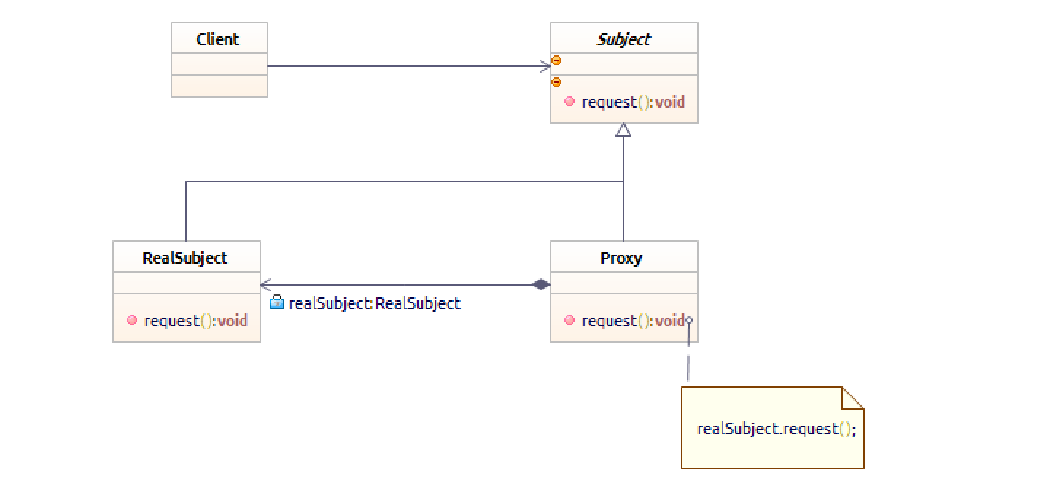
\includegraphics[width=.7\linewidth]{imagenes/Patrones/estructura_Proxy.pdf}
	\caption{Estructura del patrón Proxy.\cite{gof}}	
\end{figure}

\paragraph{Actores}

\begin{itemize}
	\item \textbf{Proxy}: Controla el acceso al sujeto real y puede ser responsable de crearlo y eliminarlo.
	\item \textbf{Sujeto}:Define la interfaz común para las clase SujetoReal y Proxy para que un Proxy se pueda usar en cualquier lugar donde se espere un SujetoReal.
	\item \textbf{Sujeto Real}:Define el objeto real al cual representa el Proxy.
\end{itemize}


\subsubsection{Caso de Uso}
